\documentclass[8pt]{beamer}
% Load Packages
\usepackage[utf8]{inputenc}
\usepackage{xcolor}
\usepackage{tikz}
\usetikzlibrary{positioning,calc}
\usepackage{graphicx}
\usepackage{hyperref}
\usepackage{amsmath}
\usepackage{listings}
\usepackage{fontawesome}

% Define Commands
\newcommand*{\ClipSep}{0.06cm} %To adjust footer logo
\newcommand{\E}{\mathrm{e}\,} % used to defined e for exp(x), see later what it should be
\newcommand{\ud}{\mathrm{d}}
\lstset{numbers=left, numberstyle=\tiny,         stepnumber=1,firstnumber=1,breaklines=true,
    numbersep=5pt,language=Python,
    stringstyle=\ttfamily,
    basicstyle=\footnotesize, 
    showstringspaces=false
}

\usetheme{oxonian}
\usepackage{amsmath}
\usepackage{fixltx2e}
\usepackage{graphicx,caption}

\newcommand*{\defeq}{\stackrel{\text{def}}{=}}
\newcommand{\newbowtie}{\mathrel{\ooalign{$\triangleright$\,\cr\,$\triangleleft$}}}
\renewcommand*\contentsname{Table of Contents}
\newcommand{\blank}[1]{\hspace*{#1}\linebreak[0]}

\title{Formal Methods Project for System Verification Project}
\subtitle{A dynamic server allocation for energy efficiency}
\titlegraphic{
\includegraphics[width=3cm]{Theme/Logos/unive.png}}
\author{Fabio Dainese (857661), Martina Donadi (865737)}
\institute{Ca' Foscari, Univeristy of Venice}
\date{December 3, 2019}

\begin{document}

{
    \setbeamertemplate{footline}{} 
    \frame{\titlepage}
}

\section*{Outline}
    \begin{frame}{Outline}
    \tableofcontents
\end{frame}

\section{Introduction}
    \begin{frame}[plain]
        \vfill
        \centering
        \begin{beamercolorbox}[sep=8pt,center,shadow=true,rounded=true]{title}
            \usebeamerfont{title}\insertsectionhead\par
            \color{univered}\noindent\rule{10cm}{1pt} \\
            \LARGE{\faFileTextO}
        \end{beamercolorbox}
        \vfill
    \end{frame}

    \begin{frame}{Problem Description}
        Power consumption in data centres receive a huge concern by data centre providers. 
        \vspace{1cm}
        \begin{itemize}
            \item Find a trade-off between performance cost and saving energy;
            \item Model a (high/low) policy to control dynamically the powering on and off of the servers.
        \end{itemize}
    \end{frame}

    \begin{frame}{Multi Server Queue Model}
        The system can basically be regarded as a multi-server queue.

        \begin{figure}[H]
            \centering
            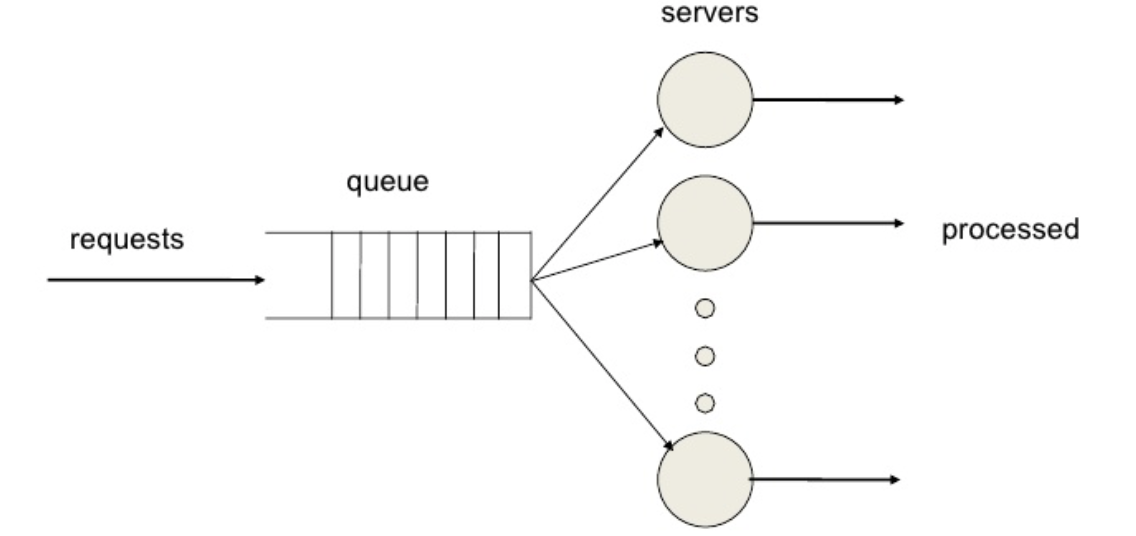
\includegraphics[width=0.6\textwidth]{Images/multi-server-queue.png}
            \caption{Multi server queue}
            \label{fig:multi-server-queue}
        \end{figure}

        \begin{itemize}
            \item N servers of which M \(<\) N static servers (always on);
            \item Alternating high/low job arrival rate.
        \end{itemize}
    \end{frame}

\section{Components and Activities of the System}
    \begin{frame}[plain]
        \vfill
        \centering
        \begin{beamercolorbox}[sep=8pt,center,shadow=true,rounded=true]{title}
            \usebeamerfont{title}\insertsectionhead\par
            \color{univered}\noindent\rule{10cm}{1pt} \\
            \LARGE{\faFileTextO}
        \end{beamercolorbox}
        \vfill
    \end{frame}

    \begin{frame}{Components of the System}
        \begin{itemize}
            \item \(Q_{i}\): Queue's current state, with \(0\leq i \leq n\), which represents the number of jobs in the system at the time \textit{i};
            \item \(Arrival_{high}\), \(Arrival_{low}\): Represent the two possible jobs' arrival stream states (high or low);
        \end{itemize}
    \end{frame}

    \begin{frame}{Components of the System}
        \begin{itemize}
            \item All the possible server's state are represented by:
            \begin{itemize}
                \item \(Server_{on}\): State in which the server is either active or idle;
                \item \(ServerPowering_{on}\): State in which the server is turning on;
                \item \(Server_{off}\): State in which the server is fully turned off;
                \item \(ServerPowering_{off}\): State in which the server is turning off;
                \item \(Server_{failOn}\): State in which the server encountered an error performing the power-up activity;
                \item \(Server_{failOff}\): State in which the server encountered an error performing the shutdown activity;
                \item \(Server_{static}\): State representing a server that is always active (\(M\) servers).
            \end{itemize}
        \end{itemize}
    \end{frame}

    \begin{frame}{Activities of the Queue}
        The set of possible actions that the \textit{queue} component can perform are:
        \vspace{1cm}
        \begin{itemize}
            \item \textbf{Service}: When a request is successfully elaborated and the job leaves the system (at a fixed rate of \(\mu\));
            \item \textbf{arrivalH}: When the arrival into the system occurs at high rate \(\lambda\);
            \item \textbf{arrivalL}: When the arrival into the system occurs at low rate \(\epsilon\).
        \end{itemize}
    \end{frame}

    \begin{frame}{Activities of the Arrival Stream}
        The activities of the \textit{arrival stream},  identified by the components \(Arrival_{high}\) and \(Arrival_{low}\), are modeled by the previously defined queue activities, i.e. \textbf{arrivalH} and \textbf{arrivalL}, and also by the switching actions between the high and low rate defined through the activities:
        \vspace{1cm}
        \begin{itemize}
            \item \textbf{highPeriodEnd} at rate \(\beta\);
            \item \textbf{lowPeriodEnd} at rate \(\gamma\).
        \end{itemize}
    \end{frame}

    \begin{frame}{Activities of the Server}
        The activities of the server are modeled by the previously defined activities \textbf{highPeriodEnd}, \textbf{lowPeriodEnd}, \textbf{service} and by new ones, such as:
        \vspace{1cm}
        \begin{itemize}
            \item \textbf{powerup}: Used to turn on a server (\(\eta\) rate);
            \item \textbf{poweroff}: Used to turn off a server (\(\xi\) rate);
            \item \textbf{repair}: Used to fix the server in case of error/fault (\(\sigma  rate\));
        \end{itemize}
    \end{frame}
 
\section{Interactions Between the Components}
    \begin{frame}{Interactions Between the Components}
        \begin{itemize}
            \item \textbf{Queue} will accept the incoming jobs, regardless the type of arrival, up until the queue if full (\(i \leq n\)), plus every time a job is served the queue index counter is decreased by 1;
            \item \textbf{Arrival Stream} will be in charge of detecting and switching accordingly to the appropriate arrival rate stream situation (high or low);
            \item \textbf{Server} will power-up or down accordingly to the high or low jobs arrival. To keep in mind that we have considered also \(M\) static servers.
        \end{itemize}
    \end{frame}

\section{PEPA Components of the System}
    \begin{frame}[plain]
        \vfill
        \centering
        \begin{beamercolorbox}[sep=8pt,center,shadow=true,rounded=true]{title}
            \usebeamerfont{title}\insertsectionhead\par
            \color{univered}\noindent\rule{10cm}{1pt} \\
            \LARGE{\faFileTextO}
        \end{beamercolorbox}
        \vfill
    \end{frame}

    \begin{frame}{Queue PEPA Component}
        \begin{align*} 
            Q_{0} &\defeq (arrivalH, \lambda).Q_{1} + (arrivalL, \epsilon).Q_{1} \\
            Q_{1} &\defeq (arrivalH, \lambda).Q_{2} + (arrivalL, \epsilon).Q_{2} + (service, \mu).Q_{1} \\
            \vdots \\
            Q_{i} &\defeq (arrivalH, \lambda).Q_{i+1} + (arrivalL, \epsilon).Q_{i+1} + (service, \mu).Q_{i-1} \\
            \vdots \\
            Q_{n} &\defeq (service, \mu).Q_{n-1}
        \end{align*}
    \end{frame}

    \begin{frame}{Queue PEPA Component}
        \begin{figure}[H]
            \centering
            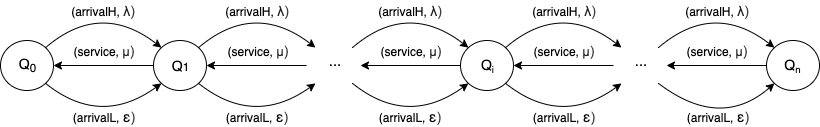
\includegraphics[width=1.0\textwidth]{Images/queue-derivation-graph.png}
            \caption{Queue PEPA derivation graph}
            \label{fig:queue-derivation-graph}
        \end{figure}
    \end{frame}
    
    \begin{frame}{Arrival Stream PEPA Component}
        \begin{align*} 
            Arrival_{high} &\defeq (arrivalH, \lambda).Arrival_{high} + (highPeriodEnd, \beta). Arrival_{low} \\
            Arrival_{low} &\defeq (arrivalL, \epsilon).Arrival_{low} + (lowPeriodEnd, \gamma). Arrival_{high}
        \end{align*} 
    \end{frame}

    \begin{frame}{Arrival Stream PEPA Component}
        \begin{figure}[H]
            \centering
            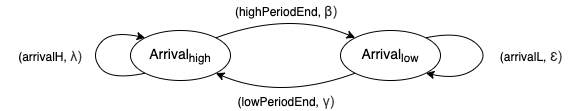
\includegraphics[width=1.0\textwidth]{Images/arrival-stream-derivation-graph.png}
            \caption{Arrival Stream PEPA derivation graph}
            \label{fig:arrival-stream-derivation-graph}
        \end{figure}
    \end{frame}

    \begin{frame}{Server PEPA Component}
        \begin{figure}[h]
            \centering
            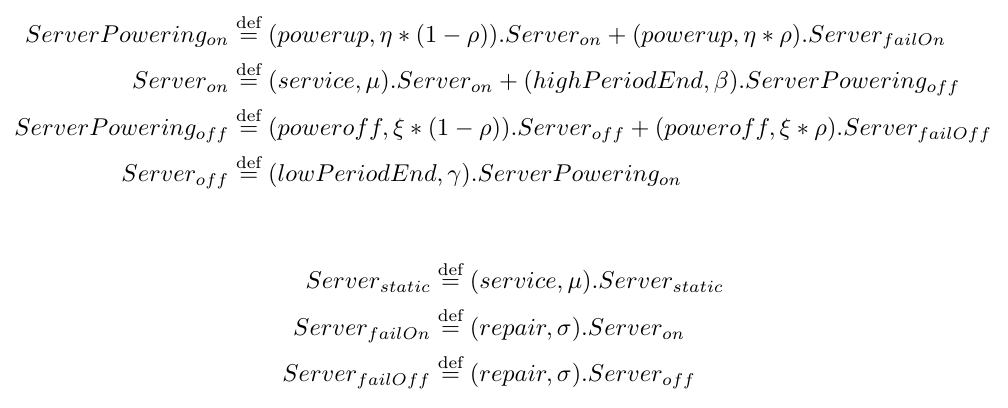
\includegraphics[width=1.0\textwidth]{Images/server-equation.png}
            \label{fig:server-equation}
        \end{figure}
    \end{frame}
    
    \begin{frame}{Server PEPA Component}
        \begin{figure}[H]
            \centering
            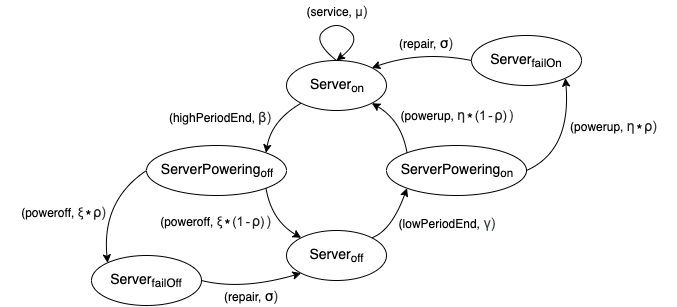
\includegraphics[width=1.0\textwidth]{Images/server-derivation-graph.png}
            \caption{Server PEPA derivation graph}
            \label{fig:server-derivation-graph}
        \end{figure}
    \end{frame}
    
    \begin{frame}{Server PEPA Component}
        \begin{figure}[H]
            \centering
            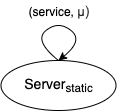
\includegraphics[width=2.5cm]{Images/server-static-derivation-graph.png}
            \caption{Static server PEPA derivation graph}
            \label{fig:server-static-derivation-graph}
        \end{figure}
    \end{frame}
    
\section{Entire System Expressed in PEPA}
    \begin{frame}[plain]
        \vfill
        \centering
        \begin{beamercolorbox}[sep=8pt,center,shadow=true,rounded=true]{title}
            \usebeamerfont{title}\insertsectionhead\par
            \color{univered}\noindent\rule{10cm}{1pt} \\
            \LARGE{\faFileTextO}
        \end{beamercolorbox}
        \vfill
    \end{frame}
    
    \begin{frame}{Entire System Expressed in PEPA}
        \[System \defeq ((Arrival_{high} \underset{K}{\newbowtie}
        Server_{on} \underset{K}{\newbowtie} ... \underset{K}{\newbowtie} Server_{on}) \underset{Z}{\newbowtie} Server_{static}[M]) \underset{L}{\newbowtie} Q_{0}\]
        
        \vspace{1cm}
        Where respectively the sets \(K,Z,L\) are defined as follows:
     
        \begin{itemize}
            \item \(K = \{highPeriodEnd\}\);
            \item \(Z = \emptyset \);
            \item \(L = \emptyset \).
        \end{itemize}
    \end{frame}

\section{Derivation Graph of the System}
    \begin{frame}[plain]
        \vfill
        \centering
        \begin{beamercolorbox}[sep=8pt,center,shadow=true,rounded=true]{title}
            \usebeamerfont{title}\insertsectionhead\par
            \color{univered}\noindent\rule{10cm}{1pt} \\
            \LARGE{\faFileTextO}
        \end{beamercolorbox}
        \vfill
    \end{frame}

    \begin{frame}{Derivation Graph}
        \[Arrival_{high} \underset{\{highPeriodEnd\}}{\newbowtie} Server_{on} \]
    
        \begin{figure}[h]
            \centering
            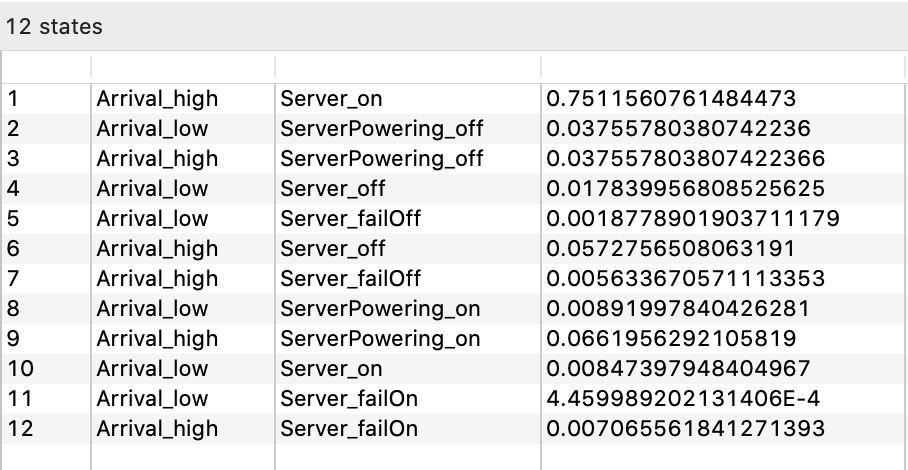
\includegraphics[width=8cm]{Images/state-space-view.png}
            \caption{Space State View for the system equation - PEPA Eclipse plug-in}
            \label{fig:space-state-view}
        \end{figure}
    \end{frame}
    
    \begin{frame}{Derivation Graph}
        \begin{figure}[H]
            \centering
            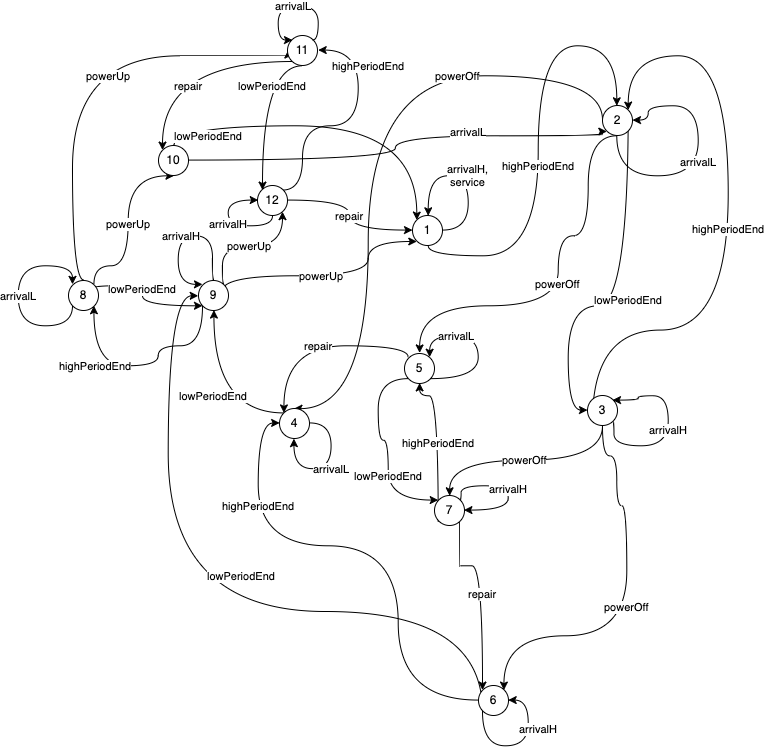
\includegraphics[width=0.65\textwidth]{Images/system-derivation-graph.png}
            \caption{System derivation graph}
            \label{fig:system-derivation-graph}
        \end{figure}
    \end{frame}

    \begin{frame}{Markov Chain}
        \begin{figure}[H]
            \centering
            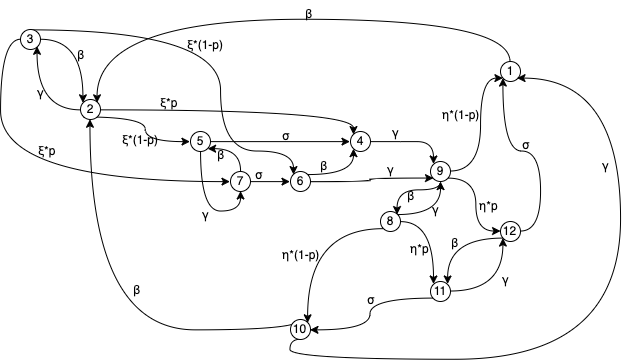
\includegraphics[width=0.8\textwidth]{Images/CTMC-representation.png}
            \caption{CTMC representation - State transition diagram}
            \label{fig:CTMC-representation}
        \end{figure}
    \end{frame}

\section{Evaluation}
    \begin{frame}[plain]
        \vfill
        \centering
        \begin{beamercolorbox}[sep=8pt,center,shadow=true,rounded=true]{title}
            \usebeamerfont{title}\insertsectionhead\par
            \color{univered}\noindent\rule{10cm}{1pt} \\
            \LARGE{\faFileTextO}
        \end{beamercolorbox}
        \vfill
    \end{frame}

    \begin{frame}{Derivation of Performance Measures}
        Different types of performance measures can be derived from the steady state distribution of a Markov Process:
        \vspace{1cm}
        \begin{itemize}
            \item State-based measures : correspond to the probability that a model is in a state (e.g. utilisation);
            \item Rate-based measures : those which correspond to the predicted rate at which some event occur (e.g. throughput);
            \item Response-time.
        \end{itemize}
    \end{frame}

    \begin{frame}{Steady State Distribution}
        When the model is in steady state we have:
        \vspace{1cm}
        \begin{itemize}
            \item the total probability flux out of each state is equal to the total probability flux into the state;
            \item \(\pi_{i}\) is the probability that the model is in state \(x_{i}\) \item \(\sum\limits_{x_{1} \in S} \pi_{i} = 1\) for \({\pi_{i}}\) is a probability distribution.
        \end{itemize}
        \vspace{1cm}
        The collection of the equations expressing the steady state condition for each state \(x_{i}\) of the model is resumed in the Global Balance equation: \[\pi Q = 0\] where Q is the Infinitesimal Generator matrix.
    \end{frame}

    \begin{frame}{Global Balance Equations}
        \begin{figure}[h]
            \centering
            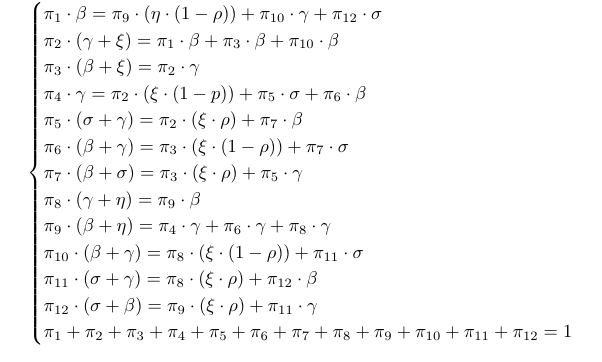
\includegraphics[width=1.0\textwidth]{Images/global-balance-system.png}
            \caption{Global balance system equations}
            \label{fig:global-balance-system}
        \end{figure}
    \end{frame}

    \begin{frame}{Infinitesimal Generator Matrix}
        \begin{figure}[h]
            \centering
            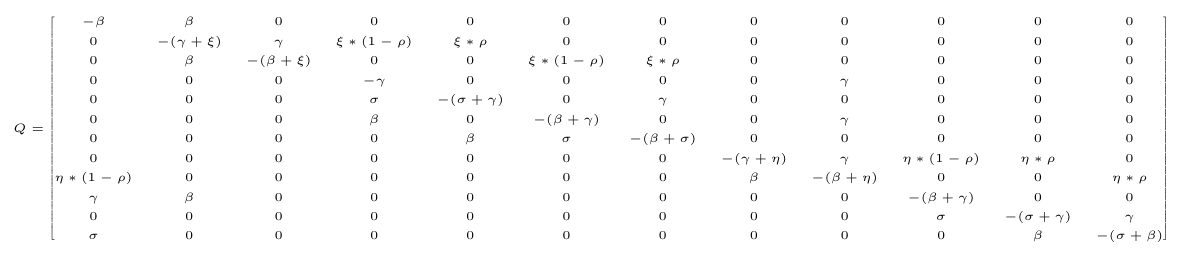
\includegraphics[width=1.0\textwidth]{Images/infinitesimal-generator-matrix.png}
            \caption{Infinitesimal generator matrix}
            \label{fig:infinitesimal-generator-matrix}
        \end{figure}
    \end{frame}
    
    \begin{frame}{Exit Rate and Sojourn Time}
        Exit rate and sojourn time are two related measures:
        \vspace{1cm}
        \begin{itemize}
            \item Exit rate: \( q_{i} = \sum\limits_{x_{j} \in S, j \neq i} q_{ij}\)
            \item Sojourn time: \( 1/q_{i}\). 
        \end{itemize}
        \vspace{1cm}
        The Sojourn time in a state \( x_{i}\) is exponentially distributed with parameter \( q_{i}\)
    \end{frame}

    \begin{frame}{Exit Rates}
        \begin{figure}[h]
            \centering
            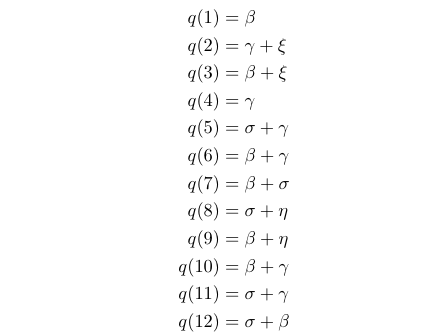
\includegraphics[width=0.8\textwidth]{Images/exit-rates.png}
            \label{fig:exit-rates}
            \caption{Exit rates}
        \end{figure}
    \end{frame}
    
    \begin{frame}{Sojourn Times}
        \begin{figure}[h]
            \centering
            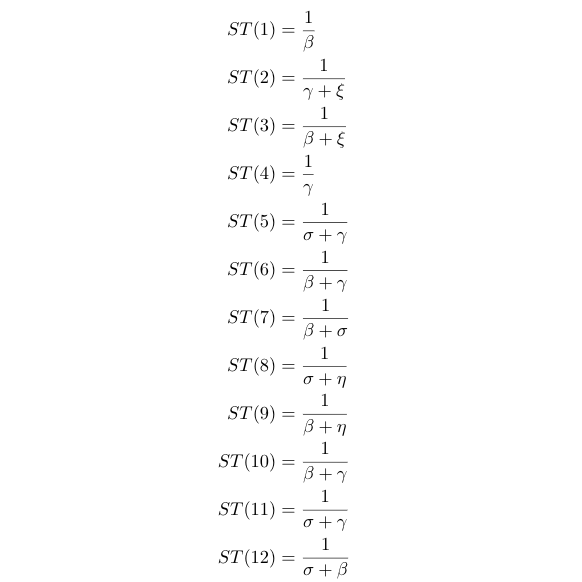
\includegraphics[width=0.6\textwidth]{Images/sojourn-times.png}
            \caption{Sojourn times}
            \label{fig:sojourn-times}
        \end{figure}
    \end{frame}
    
    \begin{frame}{Utilization}
        The \textit{utilisation} measure is the total probability that the model is in one of the states in which the resource is in use.\newline
        \[U_{Arrival_{high}} = \pi_{1} + \pi_{3} + \pi_{6} + \pi_{7} + \pi_{9} + \pi_{12}\]
        
        \[U_{Server_{on}} = \pi_{1} + \pi_{10}\]
    \end{frame}

\section{Evaluation of the System Using the PEPA Eclipse Plug-In}
    \begin{frame}[plain]
        \vfill
        \centering
        \begin{beamercolorbox}[sep=8pt,center,shadow=true,rounded=true]{title}
            \usebeamerfont{title}\insertsectionhead\par
            \color{univered}\noindent\rule{10cm}{1pt} \\
            \LARGE{\faFileTextO}
        \end{beamercolorbox}
        \vfill
    \end{frame}
    
    \begin{frame}{Evaluation of the System Using the PEPA Eclipse Plug-In}
        \begin{figure}[h]
            \centering
            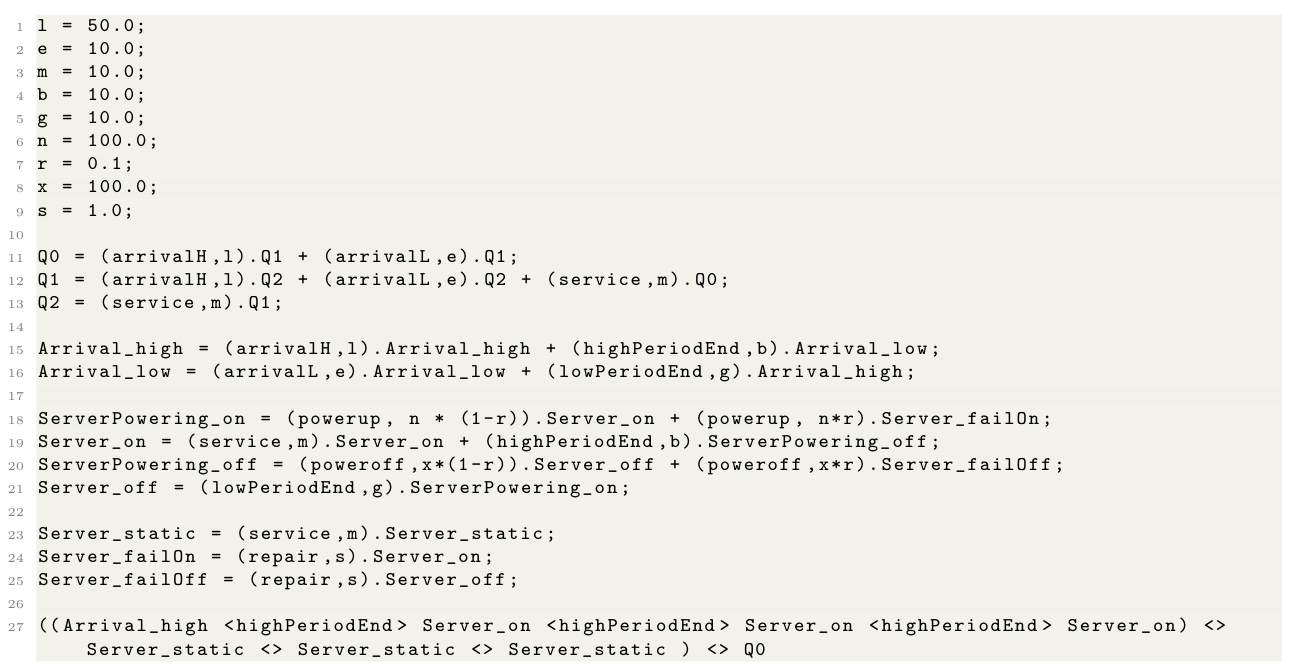
\includegraphics[width=1.0\textwidth]{Images/pepa-plugin-code.png}
            \caption{Code of the system expressed using PEPA Eclipse plug-in}
            \label{fig:pepa-plugin-code}
        \end{figure} 
    \end{frame}

    \begin{frame}{Evaluation of the System Using the PEPA Eclipse Plug-In}
        To point out that we have modeled a system having \(N = 6\) servers, which 3 of them are \textit{dynamic} and the rest are \textit{static} (i.e. always on).\newline
        For complexity reasons the queue capacity has been bounded at 2.\newline\newline
        Finally the various rates were set as follows:
        \begin{itemize}
            \item \textbf{High arrival rate}: 50;
            \item \textbf{Low arrival rate}: 10;
            \item \textbf{Powering-up and down}: 100 in equally \textit{high} and \textit{low} period of job arrivals.
        \end{itemize}
    \end{frame}

    \begin{frame}{Evaluation of the System Using the PEPA Eclipse Plug-In}
        \begin{figure}[h]
            \centering
            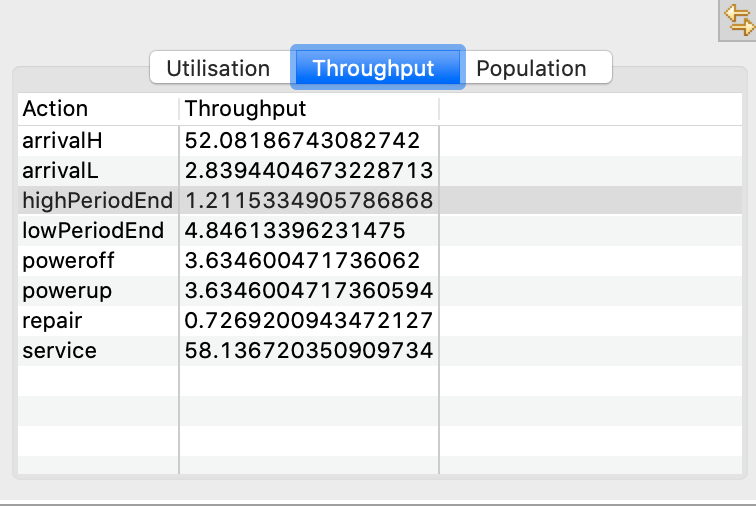
\includegraphics[width=0.8\textwidth]{Images/throughput-plugin.png}
            \caption{Throughput evaluation of the system}
            \label{fig:throughput-plugin}
        \end{figure}
    \end{frame}

    \begin{frame}{Evaluation of the System Using the PEPA Eclipse Plug-In}
        \begin{figure}[h]
            \centering
            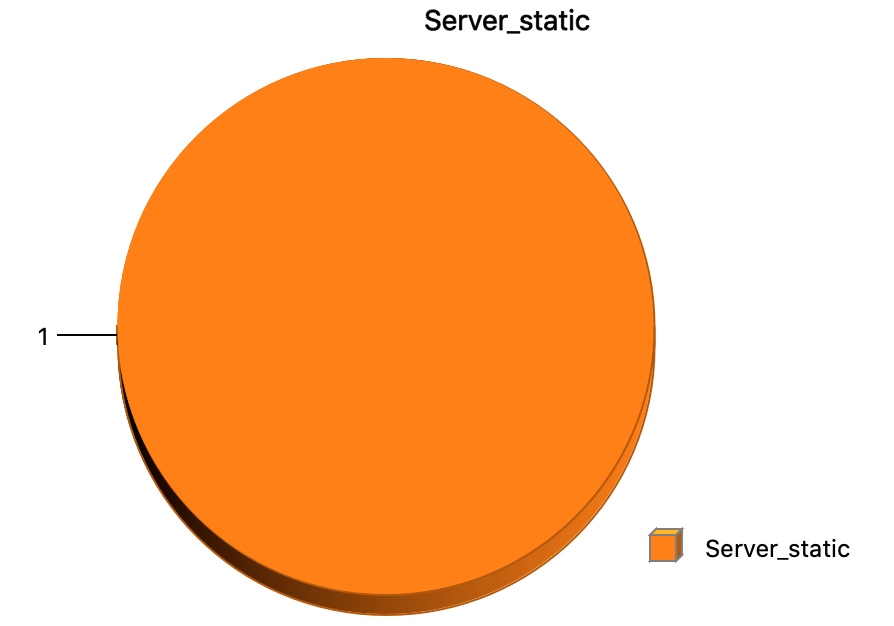
\includegraphics[width=0.8\textwidth]{Images/utilization-static-server.png}
            \caption{Utilization of the Static Server component}
            \label{fig:utilization-static-server}
        \end{figure}
    \end{frame}

    \begin{frame}{Evaluation of the System Using the PEPA Eclipse Plug-In}
        \begin{figure}[h]
            \centering
            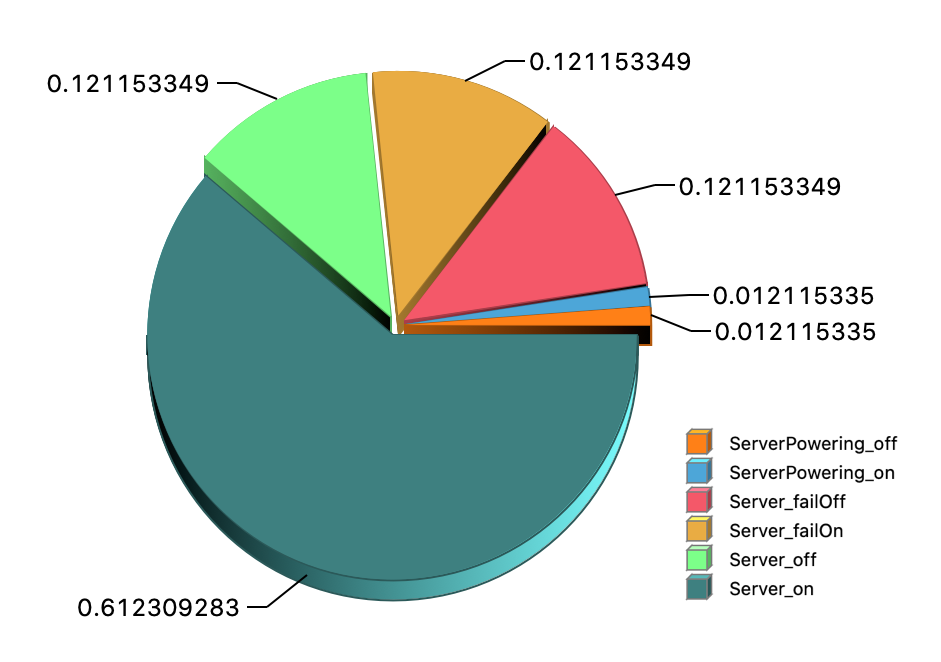
\includegraphics[width=0.8\textwidth]{Images/utilization-dynamic-server.png}
            \caption{Utilisation of the Dynamic Server component}
            \label{fig:utilization-dynamic-server}
        \end{figure}
    \end{frame}

    \begin{frame}{Evaluation of the System Using the PEPA Eclipse Plug-In}
        \begin{figure}[h]
            \centering
            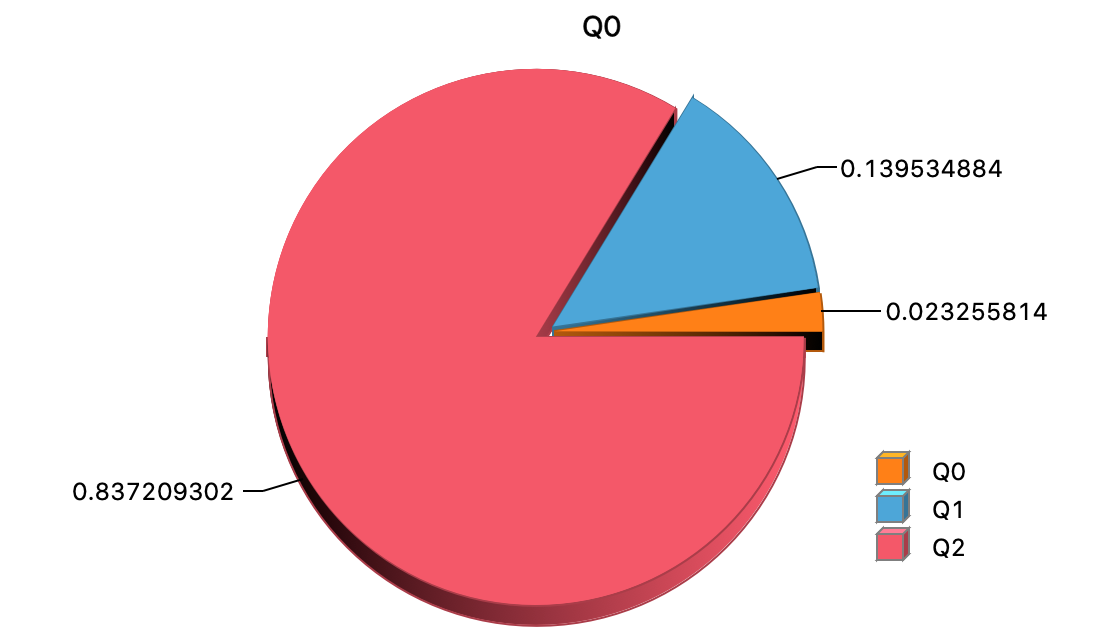
\includegraphics[width=0.8\textwidth]{Images/utilization-queue.png}
            \caption{Utilisation of the Queue component}
            \label{fig:utilization-queue}
        \end{figure}
    \end{frame}

\end{document}